\documentclass{IEEEtran}
%\usepackage[utf8]{inputenc}
\usepackage{cite}
\title{CS 6000 Journal 2}
\author{David Stout}
\date{September 7, 2018}

%\usepackage{natbib}
\usepackage{graphicx}

\begin{document}

\maketitle

\section{Process and Learning}
\subsection{The Browse}
For The Browse, I found that it was a little difficult to not read too much. I began my first few papers 
and found myself trying to read parts of the intro and conclusion to learn more about the paper to 
determine if I would want to scan it later, but after a few papers I realized that this is not the method 
that we are going for. So I tried to just do as the class slides suggested and read the abstract and scan 
the figures, then to mainly go with my gut if I was interested in the paper. I found this method to be much 
faster and really helped to weed out the papers that I just didn't really care about currently. It also 
brought to light papers that I may not care about now, but might want to read later for future research, 
which was nice to put in my notes in Zotero so that I can quickly reference them again at a later date.
\subsection{The Scan}
The scan/skim portion of reading was something that I believe came a little more naturally. I have always 
attempted to get an overall picture of what I am reading by quickly scanning each paragraph and looking for 
the key ideas, and really focusing on those ideas as well as the conclusion. I found that the timing 
recommended was just about perfect to be able to answer the six C's and the three main questions. 
\subsection{Critical read}

\begin{figure}[h!]
\centering
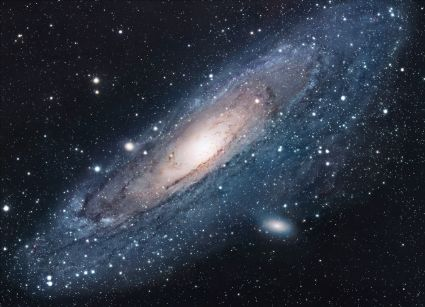
\includegraphics[scale=1.7]{universe}
\caption{The Universe}
\label{fig:universe}
\end{figure}

\section{Conclusion}


\nocite{*}

\bibliographystyle{ieeetr}
\bibliography{browsed}
\end{document}
